\documentclass[12pt]{kiarticle} % You can learn about my document class "kiarticle" and install it to your device by following the link: https://github.com/Kiarendil/toolkitex
\graphicspath{{pictures/}}
\DeclareGraphicsExtensions{.pdf,.png,.jpg,.eps}
%%%
\pagestyle{fancy}
\fancyhf{}
%\renewcommand{\headrulewidth}{ 0.1mm }
\renewcommand{\footrulewidth}{ .0em }
\fancyfoot[C]{\texttt{\textemdash~\thepage~\textemdash}}
\fancyhead[L]{Лабораторная работа № \hfil}
\fancyhead[R]{\hfil Иванов Кирилл, 625 группа }
\usepackage{multirow} % Слияние строк в таблице
\newcommand
{\un}[1]
{\ensuremath{\text{#1}}}
\newcommand{\eds}{\ensuremath{ \mathscr{E}}}
\newcommand{\ga}{\ensuremath{\gamma}}
\usepackage{tikz}
%%% Работа с таблицами
\usepackage{array,tabularx,tabulary,booktabs} % Дополнительная работа с таблицами
\usepackage{longtable}  % Длинные таблицы
\usepackage{multirow} % Слияние строк в таблице

\begin{document}
	
	\begin{titlepage}
		\begin{center}
			\large 	Московский физико-технический институт \\
			(государственный университет) \\
			Факультет общей и прикладной физики \\
			\vspace{0.2cm}
			
			\vspace{4.5cm}
			Лабораторная работа №2.2, 2.3  \\ \vspace{0.2cm}
			\large (Общая физика: квантовая физика) \\ \vspace{0.2cm}
			\LARGE \textbf{ Изучение спектров атома водорода и молекулы иона }
		\end{center}
		\vspace{2.3cm} \large
		
		\begin{center}
			Работу выполнил: \\
			Иванов Кирилл,
			625 группа
			\vspace{10mm}		
			
		\end{center}
		
		\begin{center} \vspace{60mm}
			г. Долгопрудный \\
			2018 год
		\end{center}
	\end{titlepage}


	\paragraph*{Цель работы:}  
	
	Исследовать спектральные закономерности в оптическом спектре водорода. По результатам измерений вычислить постоянную Ридберга. Исследовать спектр поглощения паров йода в видимой области; по результатам измерения вычислить энергию колебательного кванта молекулы йода и энергию ее диссоциации в основном и возбужденном состояниях.
	
	
	\section{Теоретическое введение}
	
	\subsection{Спектр водорода}
	
	Длины волн спектральных линий водородоподобного атома описываются формулой Бальмера:
	
	\begin{equation}\label{Balmer}
	\dfrac{1}{\lambda_mn} = R Z^2 \left( \dfrac{1}{n^2} - \dfrac{1}{m^2} \right) 
	\end{equation}
	
	В нашей работе изучается серия Бальмера, т.е. переходы при $ n = 2 $ и линии $ m = 3, 4, 5, 6 $, обозначаемые как $ H_\alpha, H_\beta, H_\gamma, H_\delta $.
	
	\subsection{Спектр йода}
	
	\begin{wrapfigure}[13]{l}{0.5\linewidth}
		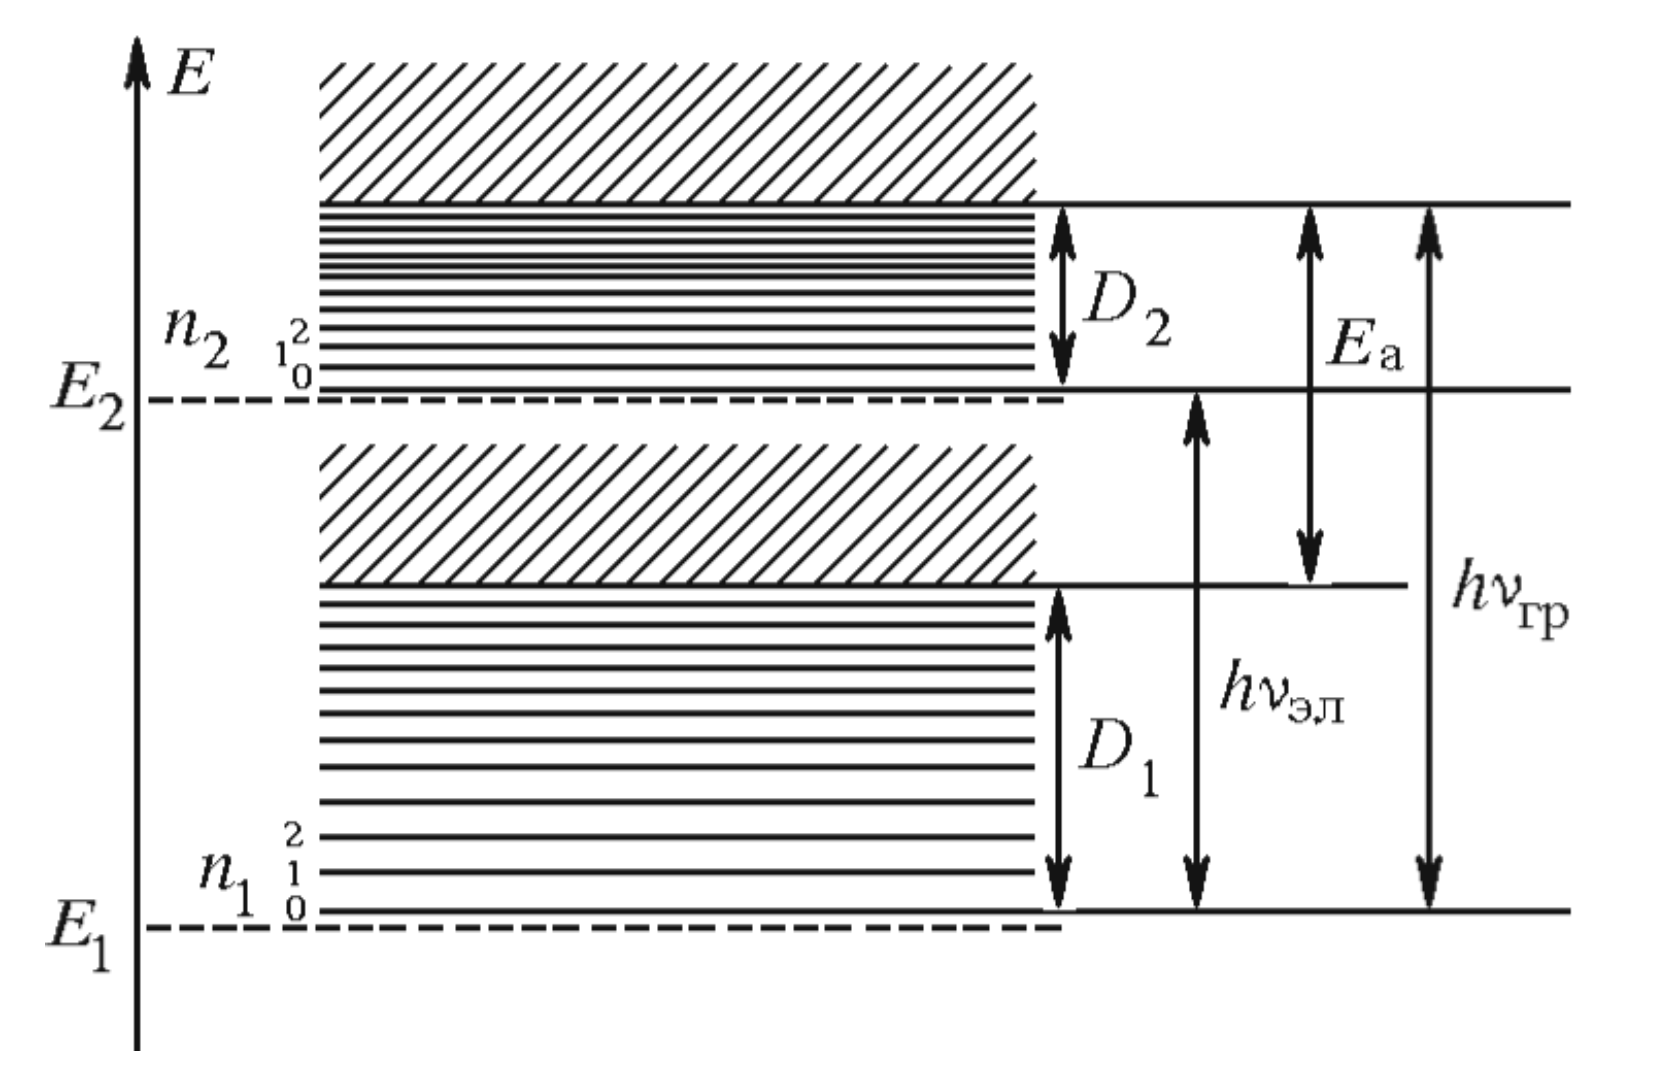
\includegraphics[width=\linewidth]{iod}
		\caption{Электронные и электронно-колебательные энергетические уровни двух-
			атомной молекулы}
		\label{ris I(V)}
	\end{wrapfigure}
	
	Оптические переходы (переходы, связанные с излучением фотонов в видимом диапазоне длин волн, т. е. фотонов с энергией порядка двух электрон-вольт) соответствуют переходам между различными электронными состояниями молекулы. При этом обычно происходят также изменения ее вращательного и колебательного состояний. 
	
	Энергетическое положение линий поглощения описывается выражением
	
	\begin{equation}\label{iod}
	h\nu_{(0,n2)} = E_2 - E_1 + h\nu_2 \left( n_2 + \dfrac{1}{2} \right) - \dfrac{h \nu_1}{2}
	\end{equation}
	
	 %TODO
	


%	\section{Экспериментальная установка}
	
	
	
	\section{Выполнение работы}
	
	Сначала выполним градуировку монохроматора. Проведем серию измерений для линий спектра неона, а затем ртути, снимая зависимость длины волны света от параметра $ \theta $ барабана монохроматора. Погрешность измерения параметра определим как $ \sigma_\theta = 5 ^\circ $ Результаты занесем в таблицу и построим график зависимости, профитировав функцию $ \lambda (\theta) $ по дисперсионной формуле Гартмана:
	
	\begin{equation}\label{labda(thta)}
	\lambda = \lambda_0 + \dfrac{C}{\theta - \theta_0}
	\end{equation}
	
	\begin{table}[H]
		\caption{Градуировка монохроматора}
		\begin{center}
			\begin{tabular}{|c|c|c|}
				\hline 
				№  линии & $ \theta $, $ ^\circ $ & $ \lambda, \;\mathring{A} $   \\ 
				\hline 
				\multicolumn{3}{|c|}{Линии спектра неона} \\
				\hline
			 1. & 7032. & 2601. \\
			2. & 6929. & 2577. \\
			3. & 6717. & 2509. \\
			4. & 6678. & 2498. \\
			5. & 6599. & 2470. \\
			6. & 6533. & 2447. \\
			7. & 6507. & 2442. \\
			8. & 6402. & 2400. \\
			9. & 6383. & 2395. \\
			10. & 6334. & 2395. \\
			11. & 6305. & 2360. \\
			12. & 6267. & 2349. \\
			13. & 6217. & 2328. \\
			14. & 6164. & 2306. \\
			15. & 6143. & 2297. \\
			16. & 6096. & 2277. \\
			17. & 6074. & 2266. \\
			18. & 6030. & 2248. \\
			19. & 5976. & 2219. \\
			20. & 5945. & 2207. \\
			21. & 5882. & 2177. \\
			22. & 5852. & 2160. \\
			23. & 5401. & 1898. \\
			24. & 5341. & 1862. \\
			25. & 5331. & 1852. \\
			\hline
				\multicolumn{3}{|c|}{Линии спектра ртути} \\
			\hline
			$ K1 $ & 6907. & 2564. \\
			$ K2 $ & 6234. & 2330. \\
			1. & 5791. & 2125. \\
			2. & 5770. & 2115. \\
			3. & 5460. & 1934. \\
			4. & 4916. & 1516. \\
			5. & 4358. & 856. \\
			6. & 4047. & 306. \\
				\hline 
			\end{tabular} 
		\end{center}
		\label{table g}
	\end{table}
	
	\begin{figure}[h!]
		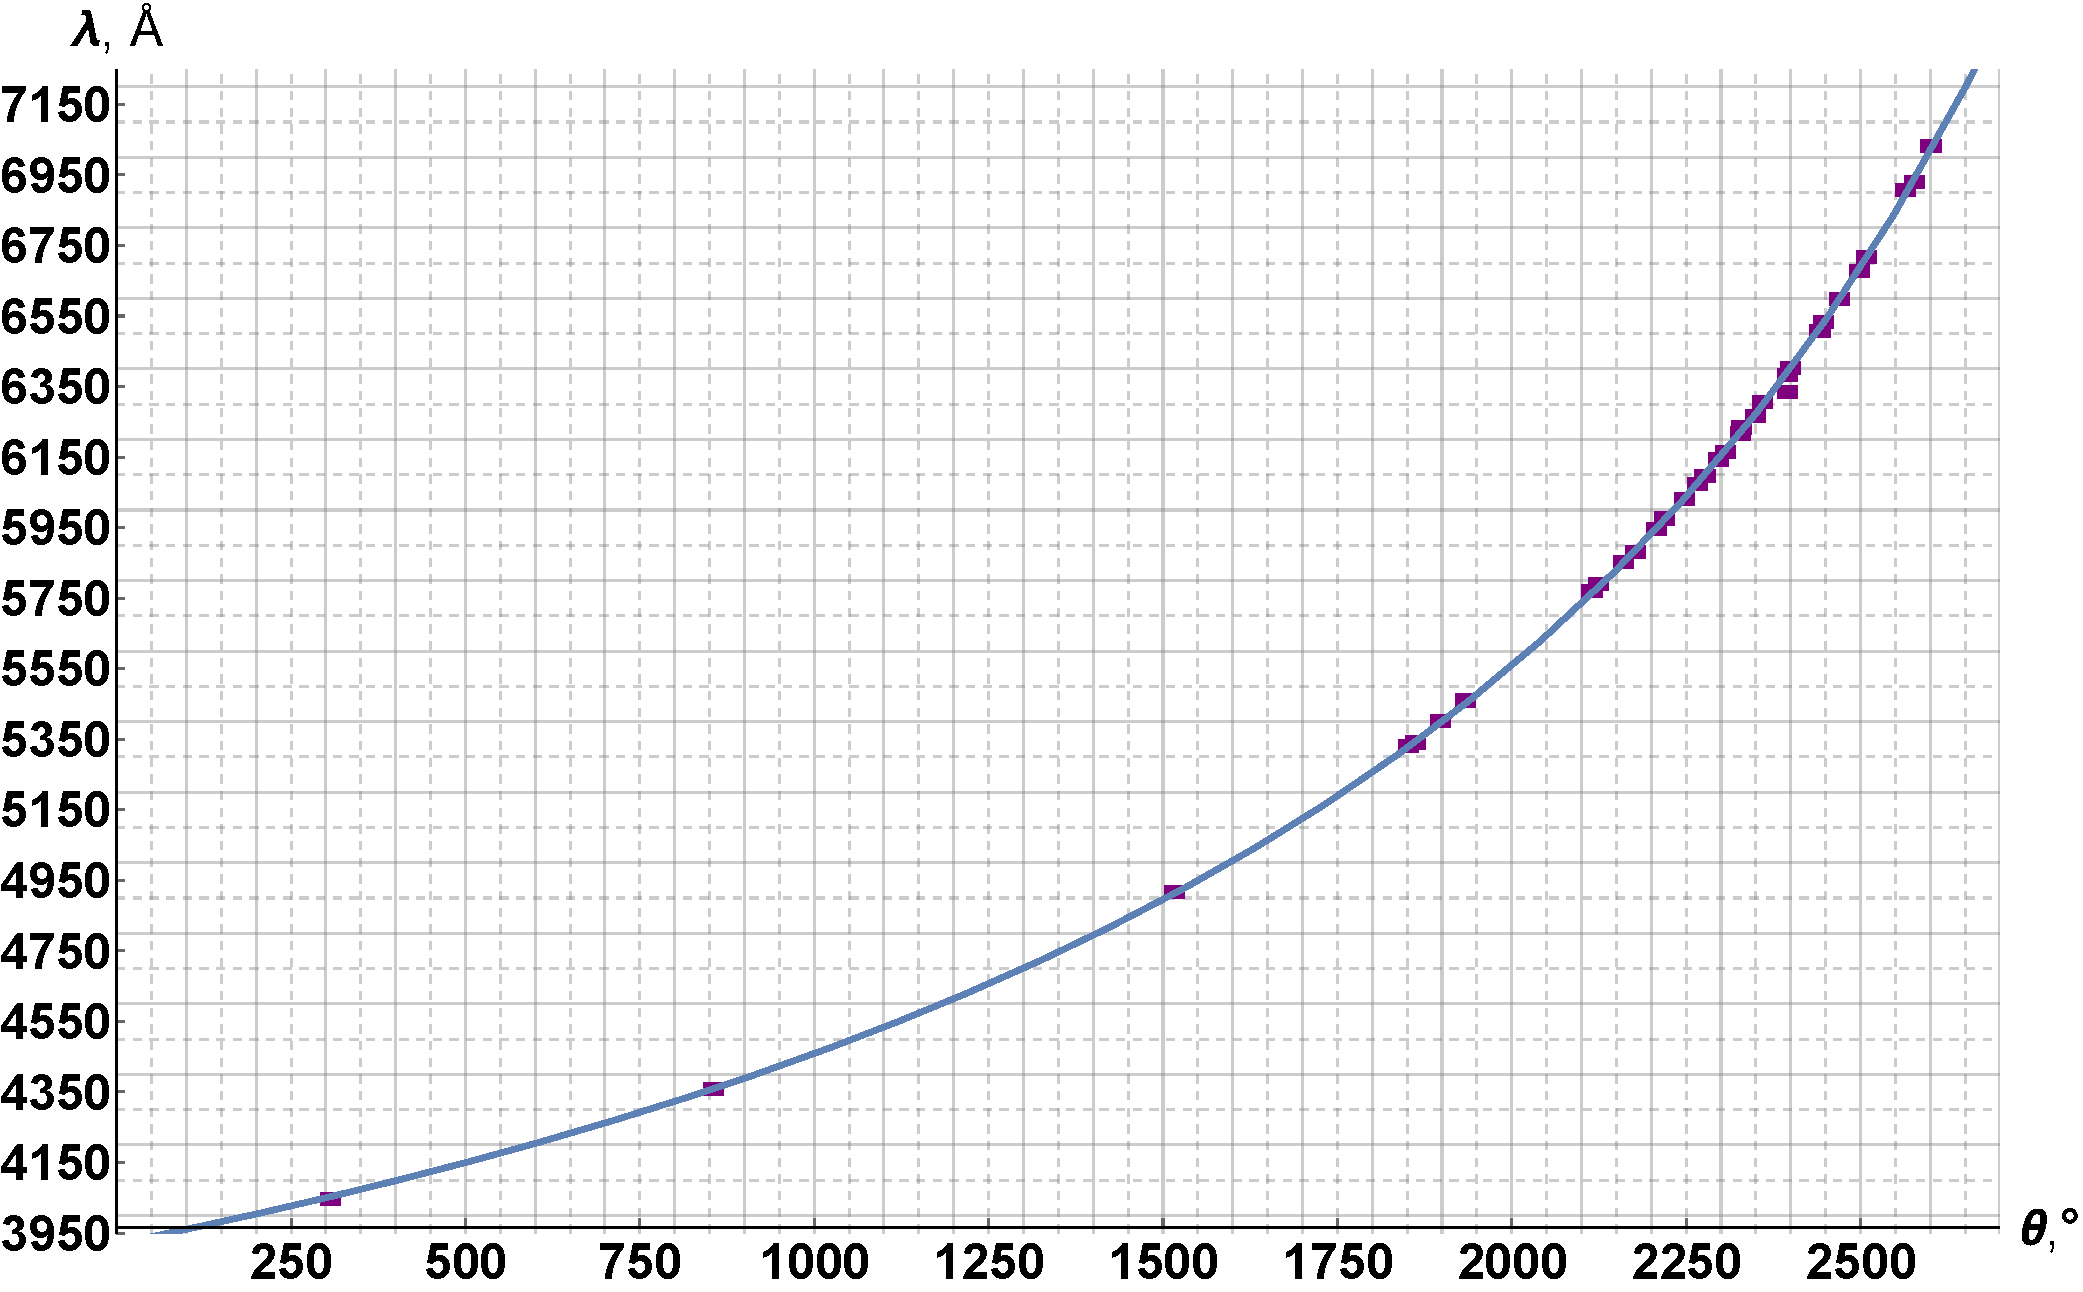
\includegraphics[scale=0.5]{G.pdf}
		\caption{Градуировка монохроматора}
		\label{graf_g}
	\end{figure} 
	
	\begin{table}[H]
		\caption{Фит рис. \ref{graf_g} функцией \eqref{labda(thta)}}
		\begin{center}
			\begin{tabular}{|c|c|c|}
				\hline
				& \text{Estimate} & \text{Standard Error} \\
				\hline
			 $ C \; [\mathring{A} \x 10^6]  $& $ -6.19  $  & $ 0.13  $ \\
			$ \theta_0 [^\circ ]$ & 3925 & 20 \\
			$ \lambda_0 [\mathring{A}] $  & 2341 & 35 \\
				\hline 
			\end{tabular} 
		\end{center}
		\label{}
	\end{table}
	
	Рассмотрим линии спектра водорода и из градуировочной кривой опеределим их длины волн. Результаты сведем в таблицу и построим график связи длины волны и номера перехода, проверяя формулу Бальмера \eqref{Balmer}:
	
		\begin{table}[h!]
		\caption{Определение линий спектра водорода}
		\begin{center}
			\begin{tabular}{|c|c|c|c|c|c|c|}
				\hline 
				Линия спектра & $ \theta $, $ ^\circ $ & $ \lambda, \;\mathring{A} $ & $ m $ & $ \frac{1}{n^2} - \frac{1}{m^2} $ & $ \frac{1}{\lambda}, \;  10^{-4} \mathring{A}^{-1} $  &  $ \sigma_{\frac{1}{\lambda}}, 10^{-4} \mathring{A}^{-1} $ \\ 
				\hline 
			$ H_\alpha $ & 2452 & 6544 & 3 & 0.139 & 1.528 & 0.046 \\
		$ H_\beta $  & 1464 & 4857 & 4 & 0.188 & 2.059 & 0.062 \\
			$ H_\gamma $ & 838 & 4347 & 5 & 0.21 & 2.3 & 0.069 \\
			$ H_\delta $ & 415 & 4105 & 6 & 0.222 & 2.436 & 0.073 \\
				\hline 
			\end{tabular} 
		\end{center}
		\label{table_mn}
	\end{table}

	\begin{figure}[h!]
		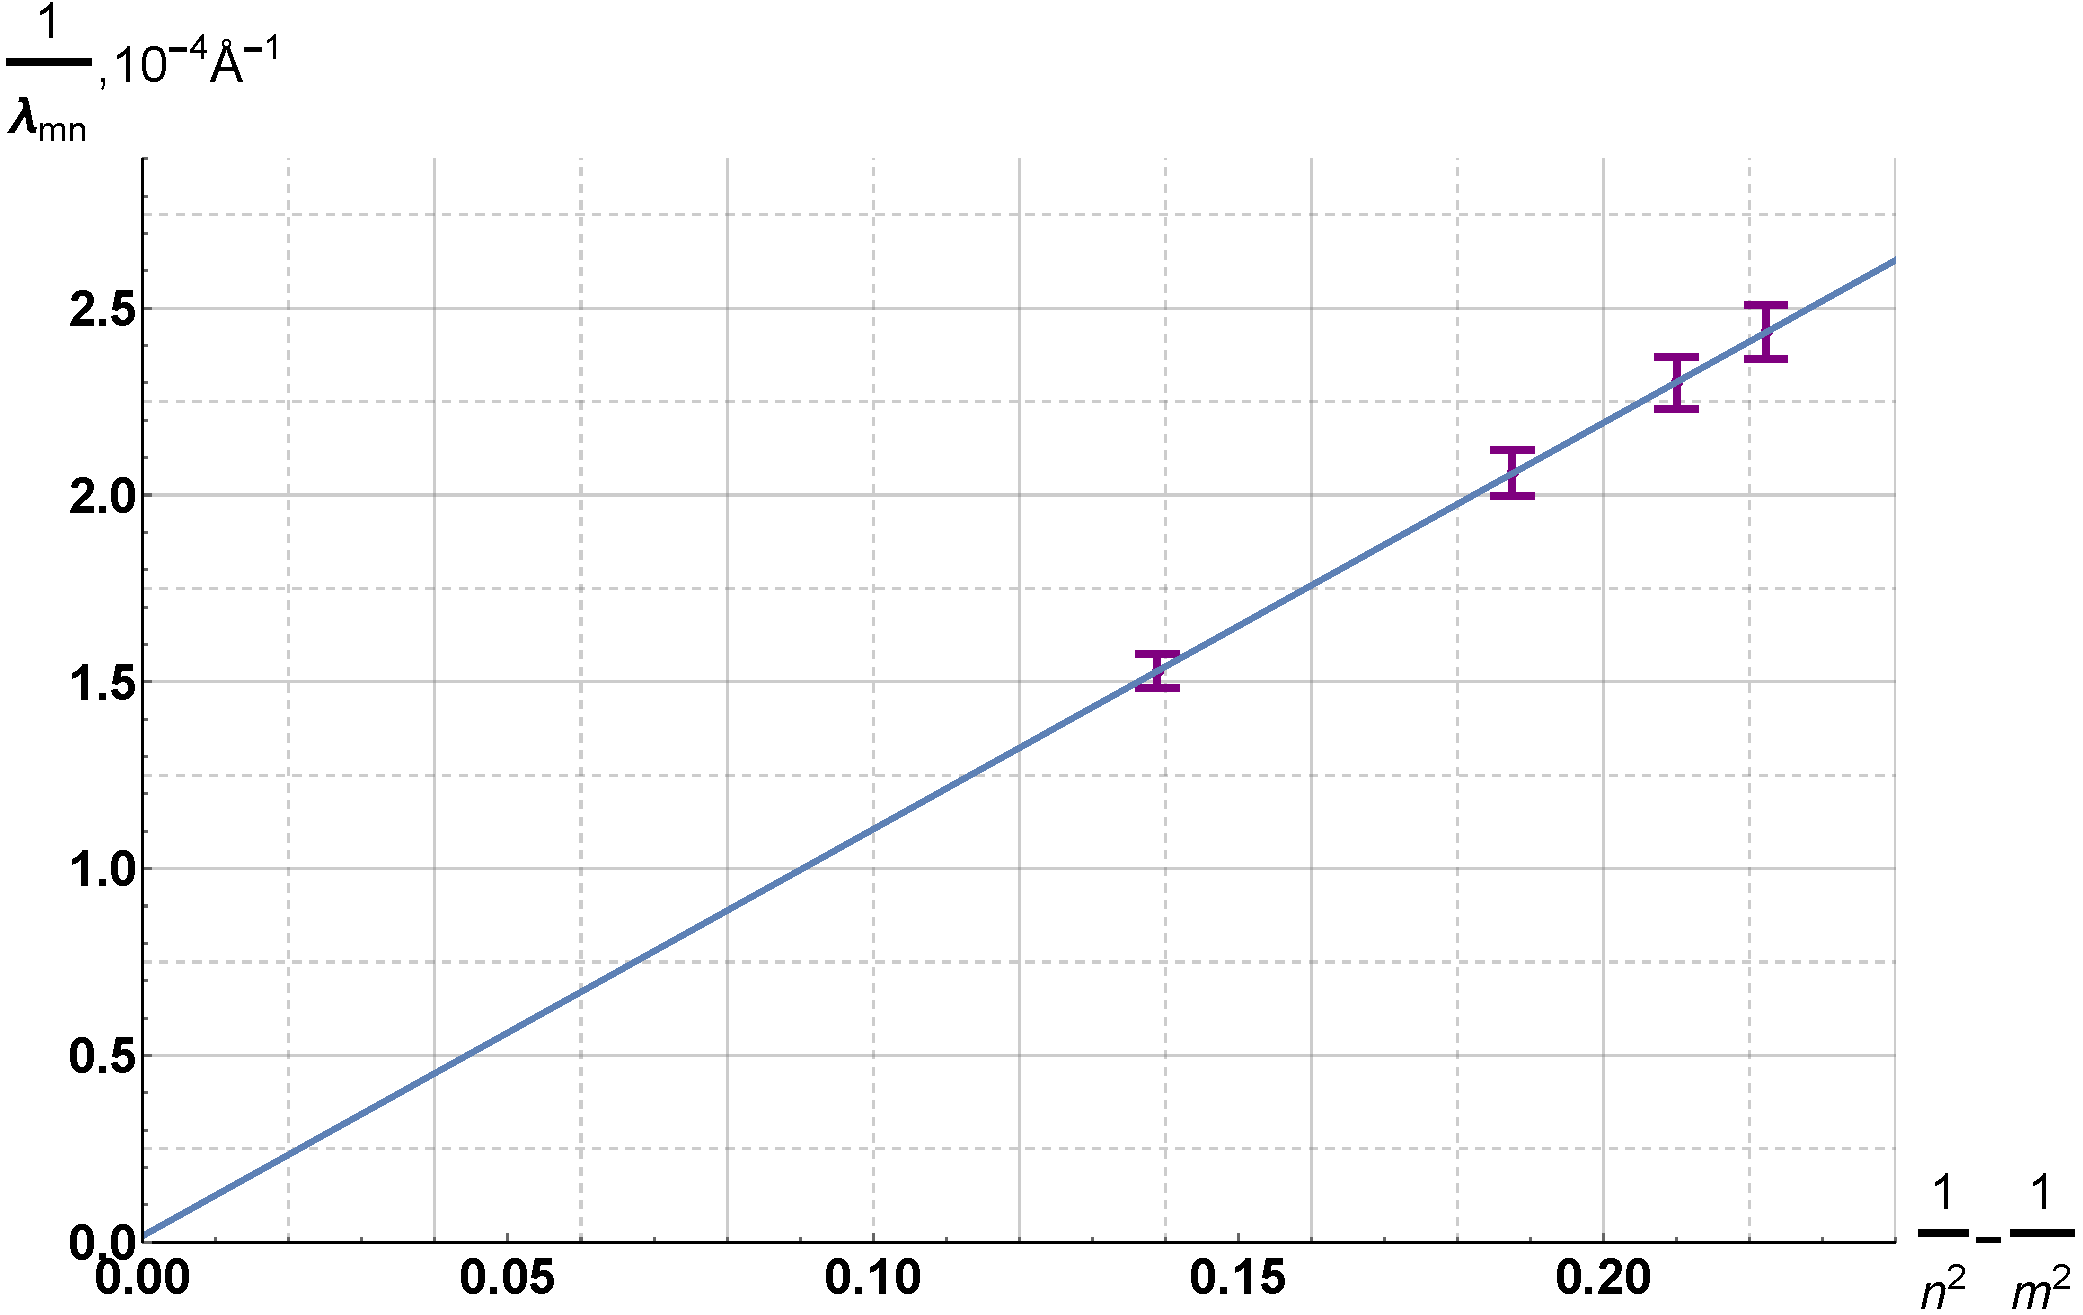
\includegraphics[scale=0.5]{mn.pdf}
		\caption{Проверка формулы Бальмера}
		\label{graf_mn}
	\end{figure} 
	
	\begin{table}[H]
		\caption{Фит рис. \ref{graf_mn} функцией $ y = ax +b $}
		\begin{center}
			\begin{tabular}{|c|c|c|}
				\hline
				& \text{Estimate} & \text{Standard Error} \\
				\hline
				 $ b $ & 0.0170 & 0.0053 \\
				$ a $& 10.9567 & 0.0276 \\
				\hline 
			\end{tabular} 
		\end{center}
%		\label{}
	\end{table}

	Отсюда можно определить постоянную Ридберга 
	
\begin{equation}\label{}
	R = (109 567 \pm 276) \; см^{-1} 
\end{equation}
	
	Теперь измерим спектр молекулы йода. Определим на монохроматоре деления, соответствующие длинноволновой линии и линии, отстоящей на 6 от нее, а также границу схождения спектра. Погрешность измерений (из фита) оценим как 1\%.
	
	\begin{enumerate}
		\item $ \theta_{1, 0} \approx 2386, \te \lambda_{1, 0} \approx 6365 \mathring{A} \te \nu_{1, 0} \approx 4,7 \x 10^{14} \; Гц \te  h \nu_{1, 0} \approx 1,95 \; эВ $
		
		\item $ \theta_{1, 5} \approx 2282, \te \lambda_{1, 5} \approx 6110 \mathring{A} \te \nu_{1, 5} \approx 4,9 \x 10^{14} \; Гц \te  h \nu_{1, 5} \approx 2,03 \; эВ $
			
		\item $ \theta_{гр} \approx 1616, \te \lambda_{гр} \approx 5023 \mathring{A} \te \nu_{гр} \approx 6,0 \x 10^{14} \; Гц \te  h \nu_{гр} \approx 2,47 \; эВ $
	\end{enumerate}

	Отсюда энергия колебательного кванта возбужденного состояния молекулы йода согласно \eqref{iod}
	
	\begin{equation}\label{}
	h\nu_2 = \dfrac{h\nu_{1, 5} - h\nu_{1, 0}}{5} = 0,0164 \pm 0,0079 \; эВ
	\end{equation}
	
	Вычислим по формуле \eqref{iod} разницу $ E_2 - E_1 = h\nu_{эл}$, сделав сдвиг серии на 1 (вычтя $ h\nu_1 $):
	
	\begin{equation}\label{}
	h \nu_{эл} = h \nu_(1,0) - \dfrac{1}{2} h\nu_2 + \dfrac{3}{2}h\nu_1 \approx 1,98  \pm 0,02 \; эВ
	\end{equation}
	
	Отсюда по рисунку рис. \ref{ris I(V)} получаем энергии диссоциации частицы в основном ($ D_1 $) и возбужденном состоянии, считая $ E_a = 0,94 $ эВ:
	
	\begin{equation}\label{}
	D_1 = h \nu_{гр} - E_a \approx 1,53 \pm 0,03 эВ, \quad D_2 = h \nu_{гр} - h \nu_{эл} \approx 0,49 \pm 0,05 \; эВ
	\end{equation}
	
	\section{Вывод }
	
	Мы изучили спектры в оптических спектрах водорода и йода, экспериментально проверили справедливость формулы Бальмера и нашли постоянную Ридберга, которая в пределах погрешность совпадает с табличной ($ R = 109 677,6 \; см^{-1} $), и оценили энергии квантов возбужденного состояния молекулы, энергию диссоциации частиц и энергию электронного перехода.
	
\end{document}
